% Options for packages loaded elsewhere
\PassOptionsToPackage{unicode}{hyperref}
\PassOptionsToPackage{hyphens}{url}
%
\documentclass[
]{article}
\usepackage{amsmath,amssymb}
\usepackage{lmodern}
\usepackage{ifxetex,ifluatex}
\ifnum 0\ifxetex 1\fi\ifluatex 1\fi=0 % if pdftex
  \usepackage[T1]{fontenc}
  \usepackage[utf8]{inputenc}
  \usepackage{textcomp} % provide euro and other symbols
\else % if luatex or xetex
  \usepackage{unicode-math}
  \defaultfontfeatures{Scale=MatchLowercase}
  \defaultfontfeatures[\rmfamily]{Ligatures=TeX,Scale=1}
\fi
% Use upquote if available, for straight quotes in verbatim environments
\IfFileExists{upquote.sty}{\usepackage{upquote}}{}
\IfFileExists{microtype.sty}{% use microtype if available
  \usepackage[]{microtype}
  \UseMicrotypeSet[protrusion]{basicmath} % disable protrusion for tt fonts
}{}
\makeatletter
\@ifundefined{KOMAClassName}{% if non-KOMA class
  \IfFileExists{parskip.sty}{%
    \usepackage{parskip}
  }{% else
    \setlength{\parindent}{0pt}
    \setlength{\parskip}{6pt plus 2pt minus 1pt}}
}{% if KOMA class
  \KOMAoptions{parskip=half}}
\makeatother
\usepackage{xcolor}
\IfFileExists{xurl.sty}{\usepackage{xurl}}{} % add URL line breaks if available
\IfFileExists{bookmark.sty}{\usepackage{bookmark}}{\usepackage{hyperref}}
\hypersetup{
  pdftitle={Assignments},
  hidelinks,
  pdfcreator={LaTeX via pandoc}}
\urlstyle{same} % disable monospaced font for URLs
\usepackage[margin=1in]{geometry}
\usepackage{color}
\usepackage{fancyvrb}
\newcommand{\VerbBar}{|}
\newcommand{\VERB}{\Verb[commandchars=\\\{\}]}
\DefineVerbatimEnvironment{Highlighting}{Verbatim}{commandchars=\\\{\}}
% Add ',fontsize=\small' for more characters per line
\usepackage{framed}
\definecolor{shadecolor}{RGB}{248,248,248}
\newenvironment{Shaded}{\begin{snugshade}}{\end{snugshade}}
\newcommand{\AlertTok}[1]{\textcolor[rgb]{0.94,0.16,0.16}{#1}}
\newcommand{\AnnotationTok}[1]{\textcolor[rgb]{0.56,0.35,0.01}{\textbf{\textit{#1}}}}
\newcommand{\AttributeTok}[1]{\textcolor[rgb]{0.77,0.63,0.00}{#1}}
\newcommand{\BaseNTok}[1]{\textcolor[rgb]{0.00,0.00,0.81}{#1}}
\newcommand{\BuiltInTok}[1]{#1}
\newcommand{\CharTok}[1]{\textcolor[rgb]{0.31,0.60,0.02}{#1}}
\newcommand{\CommentTok}[1]{\textcolor[rgb]{0.56,0.35,0.01}{\textit{#1}}}
\newcommand{\CommentVarTok}[1]{\textcolor[rgb]{0.56,0.35,0.01}{\textbf{\textit{#1}}}}
\newcommand{\ConstantTok}[1]{\textcolor[rgb]{0.00,0.00,0.00}{#1}}
\newcommand{\ControlFlowTok}[1]{\textcolor[rgb]{0.13,0.29,0.53}{\textbf{#1}}}
\newcommand{\DataTypeTok}[1]{\textcolor[rgb]{0.13,0.29,0.53}{#1}}
\newcommand{\DecValTok}[1]{\textcolor[rgb]{0.00,0.00,0.81}{#1}}
\newcommand{\DocumentationTok}[1]{\textcolor[rgb]{0.56,0.35,0.01}{\textbf{\textit{#1}}}}
\newcommand{\ErrorTok}[1]{\textcolor[rgb]{0.64,0.00,0.00}{\textbf{#1}}}
\newcommand{\ExtensionTok}[1]{#1}
\newcommand{\FloatTok}[1]{\textcolor[rgb]{0.00,0.00,0.81}{#1}}
\newcommand{\FunctionTok}[1]{\textcolor[rgb]{0.00,0.00,0.00}{#1}}
\newcommand{\ImportTok}[1]{#1}
\newcommand{\InformationTok}[1]{\textcolor[rgb]{0.56,0.35,0.01}{\textbf{\textit{#1}}}}
\newcommand{\KeywordTok}[1]{\textcolor[rgb]{0.13,0.29,0.53}{\textbf{#1}}}
\newcommand{\NormalTok}[1]{#1}
\newcommand{\OperatorTok}[1]{\textcolor[rgb]{0.81,0.36,0.00}{\textbf{#1}}}
\newcommand{\OtherTok}[1]{\textcolor[rgb]{0.56,0.35,0.01}{#1}}
\newcommand{\PreprocessorTok}[1]{\textcolor[rgb]{0.56,0.35,0.01}{\textit{#1}}}
\newcommand{\RegionMarkerTok}[1]{#1}
\newcommand{\SpecialCharTok}[1]{\textcolor[rgb]{0.00,0.00,0.00}{#1}}
\newcommand{\SpecialStringTok}[1]{\textcolor[rgb]{0.31,0.60,0.02}{#1}}
\newcommand{\StringTok}[1]{\textcolor[rgb]{0.31,0.60,0.02}{#1}}
\newcommand{\VariableTok}[1]{\textcolor[rgb]{0.00,0.00,0.00}{#1}}
\newcommand{\VerbatimStringTok}[1]{\textcolor[rgb]{0.31,0.60,0.02}{#1}}
\newcommand{\WarningTok}[1]{\textcolor[rgb]{0.56,0.35,0.01}{\textbf{\textit{#1}}}}
\usepackage{graphicx}
\makeatletter
\def\maxwidth{\ifdim\Gin@nat@width>\linewidth\linewidth\else\Gin@nat@width\fi}
\def\maxheight{\ifdim\Gin@nat@height>\textheight\textheight\else\Gin@nat@height\fi}
\makeatother
% Scale images if necessary, so that they will not overflow the page
% margins by default, and it is still possible to overwrite the defaults
% using explicit options in \includegraphics[width, height, ...]{}
\setkeys{Gin}{width=\maxwidth,height=\maxheight,keepaspectratio}
% Set default figure placement to htbp
\makeatletter
\def\fps@figure{htbp}
\makeatother
\setlength{\emergencystretch}{3em} % prevent overfull lines
\providecommand{\tightlist}{%
  \setlength{\itemsep}{0pt}\setlength{\parskip}{0pt}}
\setcounter{secnumdepth}{-\maxdimen} % remove section numbering
\ifluatex
  \usepackage{selnolig}  % disable illegal ligatures
\fi

\title{Assignments}
\author{}
\date{\vspace{-2.5em}}

\begin{document}
\maketitle

This page will contain all the assignments you submit for the class.

\hypertarget{assignment-1}{%
\section{Assignment 1}\label{assignment-1}}

\textbf{Collaborators: Theodora Athanitis and Halle Wasser }

\hypertarget{problem-1}{%
\subsubsection{Problem 1}\label{problem-1}}

Install the datasets package on the console below using
\texttt{install.packages("datasets")}. Now load the library.

\begin{Shaded}
\begin{Highlighting}[]
\CommentTok{\# install.packages(\textquotesingle{}datasets\textquotesingle{})}
\FunctionTok{library}\NormalTok{(datasets)}
\end{Highlighting}
\end{Shaded}

\emph{Answer: Installed!}

Load the USArrests dataset and rename it \texttt{dat}. Note that this
dataset comes with R, in the package datasets, so there's no need to
load data from your computer. Why is it useful to rename the dataset?

\begin{Shaded}
\begin{Highlighting}[]
\NormalTok{dat }\OtherTok{\textless{}{-}}\NormalTok{ USArrests}
\end{Highlighting}
\end{Shaded}

Answer: Renaming data sets ensures that you do not edit any of your
original data on accident, and it is also easier to type.

\hypertarget{problem-2}{%
\subsubsection{Problem 2}\label{problem-2}}

Use this command to make the state names into a new variable called
State.

\begin{Shaded}
\begin{Highlighting}[]
\NormalTok{dat}\SpecialCharTok{$}\NormalTok{state }\OtherTok{\textless{}{-}} \FunctionTok{tolower}\NormalTok{(}\FunctionTok{rownames}\NormalTok{(USArrests))}
\end{Highlighting}
\end{Shaded}

This dataset has the state names as row names, so we just want to make
them into a new variable. We also make them all lower case, because that
will help us draw a map later - the map function requires the states to
be lower case.

List the variables contained in the dataset \texttt{USArrests}.

\begin{Shaded}
\begin{Highlighting}[]
\FunctionTok{names}\NormalTok{(dat)}
\end{Highlighting}
\end{Shaded}

\begin{verbatim}
## [1] "Murder"   "Assault"  "UrbanPop" "Rape"     "state"
\end{verbatim}

\emph{Answer: The variables are Murder, Assault, Urban Population, and
Rape, in addition to the new variable that we just created, state.}

\hypertarget{problem-3}{%
\subsubsection{Problem 3}\label{problem-3}}

What type of variable (from the DVB chapter) is \texttt{Murder}?

\emph{Answer: Murder is a quantitative variable according to the DVB
chapter because we are measuring the amount of murder arrests per
100,000.}

What R Type of variable is it?

\begin{Shaded}
\begin{Highlighting}[]
\FunctionTok{class}\NormalTok{(dat}\SpecialCharTok{$}\NormalTok{Murder)}
\end{Highlighting}
\end{Shaded}

\begin{verbatim}
## [1] "numeric"
\end{verbatim}

\emph{Answer: In R, the data points in the Murder column are numeric
variables according to the class() function.}

\hypertarget{problem-4}{%
\subsubsection{Problem 4}\label{problem-4}}

What information is contained in this data set, in general? What do the
numbers mean?

\begin{Shaded}
\begin{Highlighting}[]
\FunctionTok{head}\NormalTok{(dat)}
\end{Highlighting}
\end{Shaded}

\begin{verbatim}
##            Murder Assault UrbanPop Rape      state
## Alabama      13.2     236       58 21.2    alabama
## Alaska       10.0     263       48 44.5     alaska
## Arizona       8.1     294       80 31.0    arizona
## Arkansas      8.8     190       50 19.5   arkansas
## California    9.0     276       91 40.6 california
## Colorado      7.9     204       78 38.7   colorado
\end{verbatim}

\begin{Shaded}
\begin{Highlighting}[]
\StringTok{\textasciigrave{}}\AttributeTok{?}\StringTok{\textasciigrave{}}\NormalTok{(USArrests)}
\end{Highlighting}
\end{Shaded}

\emph{Answer: Generally, this data set contains rates for specific crime
arrests per 100,000 people collected by D.R. McNeil, as well as
percentages of urban population per state in 1973. The numbers in the
Murder, Assault, and Rape columns are equivalent to the calculated
arrest rates for Murder, Assault, and Rape. The Urban Population numbers
are the percentages of the population in each state that live in an
urban area.}

\hypertarget{problem-5}{%
\subsubsection{Problem 5}\label{problem-5}}

Draw a histogram of \texttt{Murder} with proper labels and title.

\begin{Shaded}
\begin{Highlighting}[]
\FunctionTok{hist}\NormalTok{(dat}\SpecialCharTok{$}\NormalTok{Murder, }\AttributeTok{xlab =} \StringTok{"Murder Arrests per 100,000 People"}\NormalTok{,}
    \AttributeTok{main =} \StringTok{"Frequency of Murder Arrest Rates in the US"}\NormalTok{, }\AttributeTok{col =} \StringTok{"purple"}\NormalTok{)}
\end{Highlighting}
\end{Shaded}

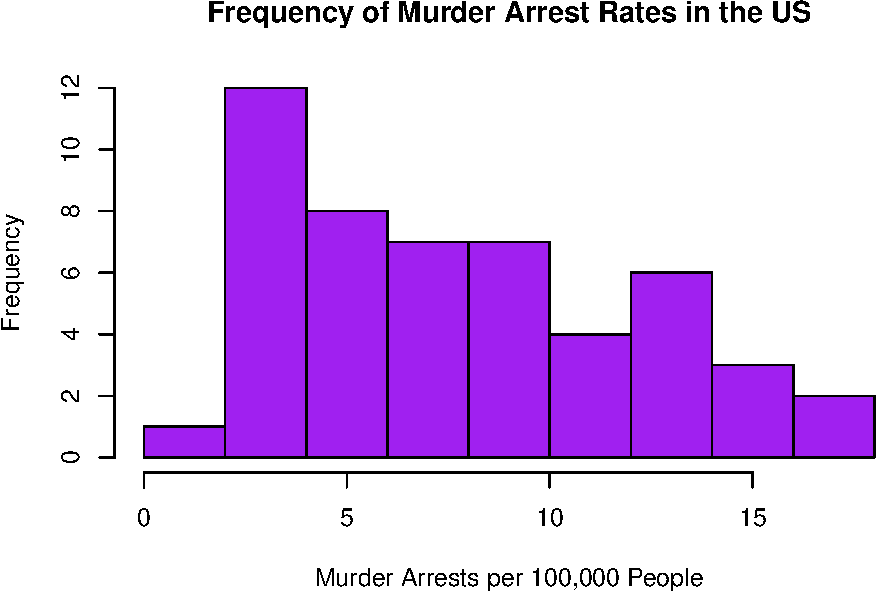
\includegraphics{Assignments_files/figure-latex/unnamed-chunk-7-1.pdf}

\hypertarget{problem-6}{%
\subsubsection{Problem 6}\label{problem-6}}

Please summarize \texttt{Murder} quantitatively. What are its mean and
median? What is the difference between mean and median? What is a
quartile, and why do you think R gives you the 1st Qu. and 3rd Qu.?

\begin{Shaded}
\begin{Highlighting}[]
\FunctionTok{summary}\NormalTok{(dat}\SpecialCharTok{$}\NormalTok{Murder)}
\end{Highlighting}
\end{Shaded}

\begin{verbatim}
##    Min. 1st Qu.  Median    Mean 3rd Qu.    Max. 
##   0.800   4.075   7.250   7.788  11.250  17.400
\end{verbatim}

\emph{Answer: The mean is 7.788. The median is 7.250. Q1 is 4.075 and Q3
is 11.250. The minimum value is .800 and the maximum value is 17.400.
Mean and median are both measures of center; however, the mean is the
average value of a data set, which is calculated by adding all of the
values and dividing by the number of total data points, and the mean is
calculated by finding the middle value when the data set is arranged in
order. A quartile is essentially the same as a median, but with 25\% and
75\% of the data, rather than 50\%. This means that 25\% of the data in
a data set is below the 1st quartile, 50\% is below the second quartile
(the median), and 75\% is below the 3rd quartile. R gives you quartiles
in order to help visualize the data and see if it is distributed
symmetrically, and only gives you quartiles 1 and 3 because the median
is the 2nd quartile.}

\hypertarget{problem-7}{%
\subsubsection{Problem 7}\label{problem-7}}

Repeat the same steps you followed for \texttt{Murder}, for the
variables \texttt{Assault} and \texttt{Rape}. Now plot all three
histograms together. You can do this by using the command
\texttt{par(mfrow=c(3,1))} and then plotting each of the three.

\begin{Shaded}
\begin{Highlighting}[]
\FunctionTok{hist}\NormalTok{(dat}\SpecialCharTok{$}\NormalTok{Assault, }\AttributeTok{xlab =} \StringTok{"Assault Arrests per 100,000 People"}\NormalTok{,}
    \AttributeTok{main =} \StringTok{"Frequency of Assault Arrest Rates in the US"}\NormalTok{, }\AttributeTok{col =} \StringTok{"Blue"}\NormalTok{)}
\end{Highlighting}
\end{Shaded}

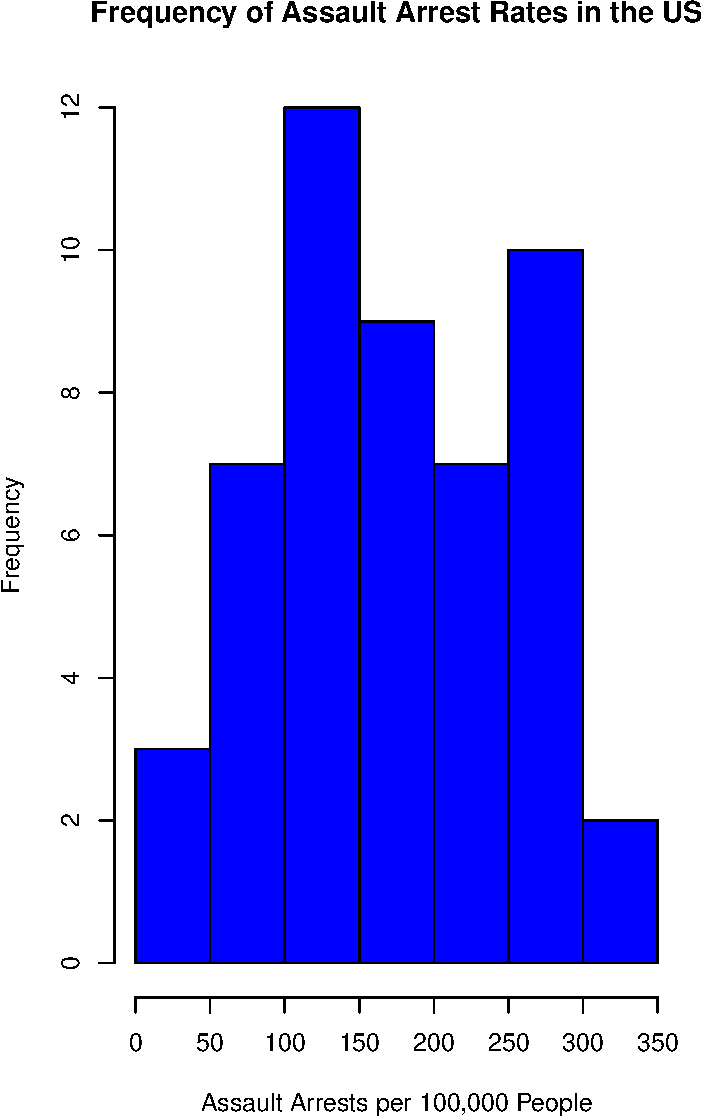
\includegraphics{Assignments_files/figure-latex/unnamed-chunk-9-1.pdf}

\begin{Shaded}
\begin{Highlighting}[]
\FunctionTok{summary}\NormalTok{(dat}\SpecialCharTok{$}\NormalTok{Assault)}
\end{Highlighting}
\end{Shaded}

\begin{verbatim}
##    Min. 1st Qu.  Median    Mean 3rd Qu.    Max. 
##    45.0   109.0   159.0   170.8   249.0   337.0
\end{verbatim}

\emph{Answer: The mean is 170.8. The median is 159.0. Q1 is 109.0 and Q3
is 249.0. The minimum value is 45.0 and the maximum value is 337.0.}

\begin{Shaded}
\begin{Highlighting}[]
\FunctionTok{hist}\NormalTok{(dat}\SpecialCharTok{$}\NormalTok{Rape, }\AttributeTok{xlab =} \StringTok{"Rape Arrests per 100,000 People"}\NormalTok{, }\AttributeTok{main =} \StringTok{"Frequency of Rape Arrest Rates in the US"}\NormalTok{,}
    \AttributeTok{col =} \StringTok{"Red"}\NormalTok{)}
\end{Highlighting}
\end{Shaded}

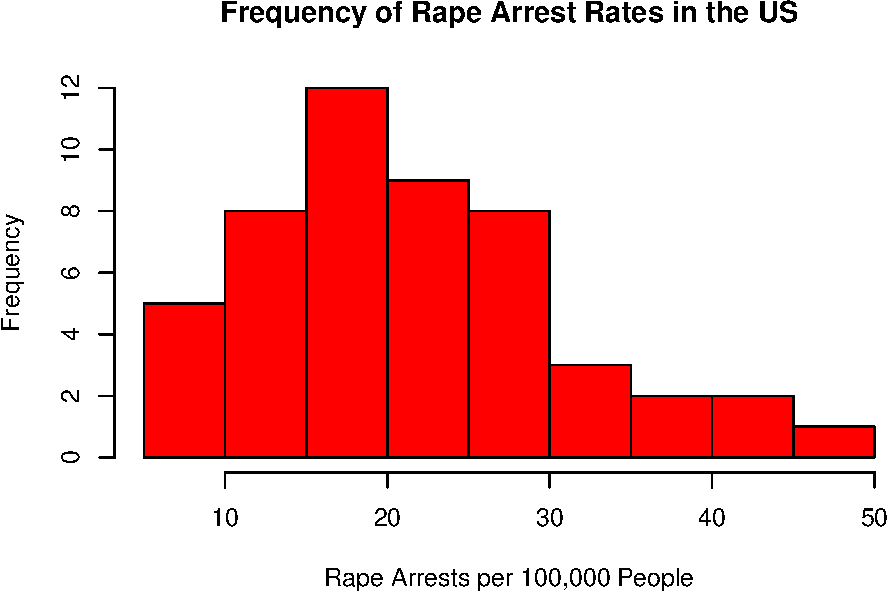
\includegraphics{Assignments_files/figure-latex/unnamed-chunk-11-1.pdf}

\begin{Shaded}
\begin{Highlighting}[]
\FunctionTok{summary}\NormalTok{(dat}\SpecialCharTok{$}\NormalTok{Rape)}
\end{Highlighting}
\end{Shaded}

\begin{verbatim}
##    Min. 1st Qu.  Median    Mean 3rd Qu.    Max. 
##    7.30   15.07   20.10   21.23   26.18   46.00
\end{verbatim}

\emph{Answer: The mean is 21.23. The median is 20.10. Q1 is 15.07 and Q3
is 26.18. The minimum value is 7.30 and the maximum value is 46.00.}

\begin{Shaded}
\begin{Highlighting}[]
\FunctionTok{par}\NormalTok{(}\AttributeTok{mfrow =} \FunctionTok{c}\NormalTok{(}\DecValTok{3}\NormalTok{, }\DecValTok{1}\NormalTok{))}
\FunctionTok{hist}\NormalTok{(dat}\SpecialCharTok{$}\NormalTok{Murder, }\AttributeTok{xlab =} \StringTok{"Murder Arrests per 100,000 People"}\NormalTok{,}
    \AttributeTok{main =} \StringTok{"Frequency of Murder Arrest Rates in the US"}\NormalTok{, }\AttributeTok{col =} \StringTok{"purple"}\NormalTok{)}
\FunctionTok{hist}\NormalTok{(dat}\SpecialCharTok{$}\NormalTok{Assault, }\AttributeTok{xlab =} \StringTok{"Assault Arrests per 100,000 People"}\NormalTok{,}
    \AttributeTok{main =} \StringTok{"Frequency of Assault Arrest Rates in the US"}\NormalTok{, }\AttributeTok{col =} \StringTok{"Blue"}\NormalTok{)}
\FunctionTok{hist}\NormalTok{(dat}\SpecialCharTok{$}\NormalTok{Rape, }\AttributeTok{xlab =} \StringTok{"Rape Arrests per 100,000 People"}\NormalTok{, }\AttributeTok{main =} \StringTok{"Frequency of Rape Arrest Rates in the US"}\NormalTok{,}
    \AttributeTok{col =} \StringTok{"Red"}\NormalTok{)}
\end{Highlighting}
\end{Shaded}

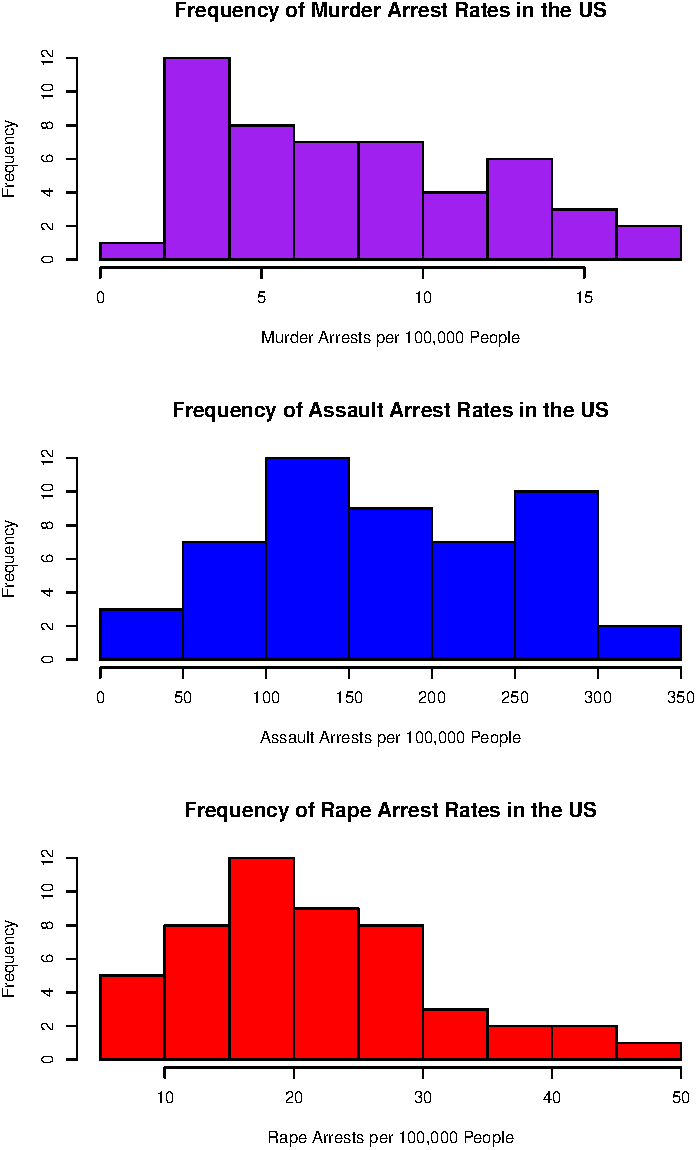
\includegraphics{Assignments_files/figure-latex/unnamed-chunk-13-1.pdf}

What does the command par do, in your own words (you can look this up by
asking R \texttt{?par})?

\emph{Answer: The `par' command sets parameters for graphs, changes how
they are displayed, and allows us to tell R to compare additional
variables within the data set. `mfrow' puts things in an array, and the
parameters of (1,3) tell it to display them stacked on top of each
other, rather than side by side or otherwise.}

What can you learn from plotting the histograms together?

\emph{Answer: We can learn that assault arrest rates per 100,000 people
are far higher than the arrest rates for murder and rape by comparing
the x axis of all three histograms. Additionally, while the frequency of
arrest rates for rape and murder skew relatively right and are unimodal,
the frequency of assault arrest rates is bimodal. Comparing and plotting
them together can generally help us visually compare distributions
overall.}

\hypertarget{problem-8}{%
\subsubsection{Problem 8}\label{problem-8}}

In the console below (not in text), type
\texttt{install.packages("maps")} and press Enter, and then type
\texttt{install.packages("ggplot2")} and press Enter. This will install
the packages so you can load the libraries.

Run this code:

\begin{Shaded}
\begin{Highlighting}[]
\CommentTok{\# install.packages(\textquotesingle{}maps\textquotesingle{}) install.packages(\textquotesingle{}ggplot2\textquotesingle{})}
\FunctionTok{library}\NormalTok{(}\StringTok{"maps"}\NormalTok{)}
\FunctionTok{library}\NormalTok{(}\StringTok{"ggplot2"}\NormalTok{)}

\FunctionTok{ggplot}\NormalTok{(dat, }\FunctionTok{aes}\NormalTok{(}\AttributeTok{map\_id =}\NormalTok{ state, }\AttributeTok{fill =}\NormalTok{ Murder)) }\SpecialCharTok{+} \FunctionTok{geom\_map}\NormalTok{(}\AttributeTok{map =} \FunctionTok{map\_data}\NormalTok{(}\StringTok{"state"}\NormalTok{)) }\SpecialCharTok{+}
    \FunctionTok{expand\_limits}\NormalTok{(}\AttributeTok{x =} \FunctionTok{map\_data}\NormalTok{(}\StringTok{"state"}\NormalTok{)}\SpecialCharTok{$}\NormalTok{long, }\AttributeTok{y =} \FunctionTok{map\_data}\NormalTok{(}\StringTok{"state"}\NormalTok{)}\SpecialCharTok{$}\NormalTok{lat)}
\end{Highlighting}
\end{Shaded}

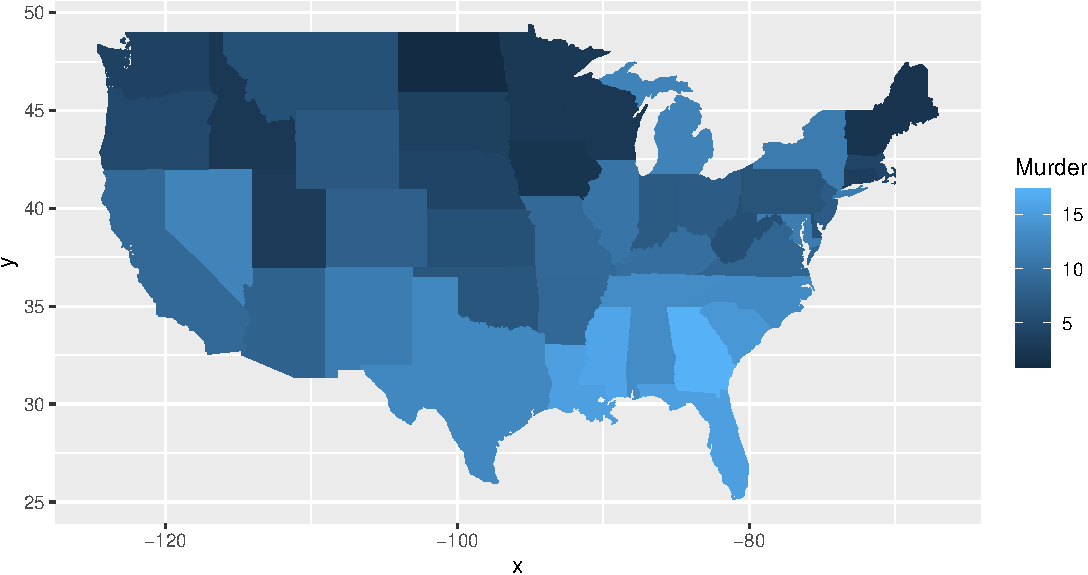
\includegraphics{Assignments_files/figure-latex/unnamed-chunk-14-1.pdf}

What does this code do? Explain what each line is doing.

\emph{Answer:}

\begin{Shaded}
\begin{Highlighting}[]
\CommentTok{\# install.packages(\textquotesingle{}maps\textquotesingle{})}
\CommentTok{\#{-} This line installs a package that allows for map{-}drawing based on state names provided within the data.}
\CommentTok{\# install.packages(\textquotesingle{}ggplot2\textquotesingle{})}
\CommentTok{\#{-} This line installs a package that makes improves the data visualization so that the map is easier to understand.}
\CommentTok{\# library(\textquotesingle{}maps\textquotesingle{})}
\CommentTok{\#{-} This line tells R where to find the package to help draw the map}
\CommentTok{\# library(\textquotesingle{}ggplot2\textquotesingle{})}
\CommentTok{\#{-} This line tells R where to find the package to help draw the map}
\CommentTok{\# ggplot(dat, aes(map\_id=state, fill=Murder)) +}
\CommentTok{\# geom\_map(map=map\_data(\textquotesingle{}state\textquotesingle{})) +}
\CommentTok{\# expand\_limits(x=map\_data(\textquotesingle{}state\textquotesingle{})$long,}
\CommentTok{\# y=map\_data(\textquotesingle{}state\textquotesingle{})$lat)}
\CommentTok{\#{-} This line tells R to use ggplot and to take information from dat variable \textquotesingle{}state\textquotesingle{}, and then to draw a map with US states, specifically using numbers from the Murder column. This line also instructs R to color each state based on the numbers in the \textquotesingle{}Murder\textquotesingle{} column. It additionally tells R to make the x and y axes and limits align with longitude and latitude in a US map.}
\end{Highlighting}
\end{Shaded}

\hypertarget{assignment-2}{%
\section{Assignment 2}\label{assignment-2}}

\textbf{Collaborators: Theodora Athanitis}

\hypertarget{problem-1-1}{%
\subsubsection{Problem 1}\label{problem-1-1}}

\emph{Instructions: Copy your code, paste it into a Word document, and
turn it into Canvas. You can turn in a .docx or .pdf file. Show any EDA
(graphical or non-graphical) you have used to come to this conclusion.}

Problem 1: Load data

Set your working directory to the folder where you downloaded the data.

\begin{Shaded}
\begin{Highlighting}[]
\FunctionTok{setwd}\NormalTok{(}\StringTok{"/Users/toriborlase/Desktop/University of Pennsylvania/Fall 2021/CRIM 250/Tori{-}Borlase{-}Crim{-}250"}\NormalTok{)}
\end{Highlighting}
\end{Shaded}

Read the data

\begin{Shaded}
\begin{Highlighting}[]
\NormalTok{dat }\OtherTok{\textless{}{-}} \FunctionTok{read.csv}\NormalTok{(}\AttributeTok{file =} \StringTok{"dat.nsduh.small.1.csv"}\NormalTok{)}
\end{Highlighting}
\end{Shaded}

What are the dimensions of the dataset?

\begin{Shaded}
\begin{Highlighting}[]
\FunctionTok{dim}\NormalTok{(dat)}
\end{Highlighting}
\end{Shaded}

\begin{verbatim}
## [1] 171   7
\end{verbatim}

Answer: 171 by 7. 171 rows and 7 columns.

\hypertarget{problem-2-variables}{%
\subsubsection{Problem 2: Variables}\label{problem-2-variables}}

Describe the variables in the dataset.

\begin{Shaded}
\begin{Highlighting}[]
\FunctionTok{names}\NormalTok{(dat)}
\end{Highlighting}
\end{Shaded}

\begin{verbatim}
## [1] "mjage"     "cigage"    "iralcage"  "age2"      "sexatract" "speakengl"
## [7] "irsex"
\end{verbatim}

\emph{Answer: The variables in the dataset are mjage, cigage, iralcage,
age2, sexatract, speakengl, and irsex. According to the code book, these
correspond to how old someone was when they first tried marijuana or
hashish, how old someone was when they started smoking cigarettes every
day, how old someone was when they first tried alcohol, the final age
that someone was determined to be at the time of taking the survey
(which was asked multiple times as a consistency check), which statement
about sexual orientation best described the respondent's feelings, how
well they speak English, and imputation revised gender.}

What is this dataset about? Who collected the data, what kind of sample
is it, and what was the purpose of generating the data?

\emph{Answer: This dataset is from the 2019 National Survey on Drug Use
and Health (NSDUH). Individuals within the Center for Behavioral Health
Statistics and Quality collected this data in order to measure the
``prevalence and correlates of substance use and mental health issues''
in the US. This was a stratified random sample, as they collected data
in all 50 states for civilian and non-institutionalized populations.}

\hypertarget{problem-3-age-and-gender}{%
\subsection{Problem 3: Age and gender}\label{problem-3-age-and-gender}}

What is the age distribution of the sample like? Make sure you read the
codebook to know what the variable values mean.

\begin{Shaded}
\begin{Highlighting}[]
\NormalTok{counts }\OtherTok{\textless{}{-}} \FunctionTok{table}\NormalTok{(dat}\SpecialCharTok{$}\NormalTok{age2)}
\FunctionTok{barplot}\NormalTok{(counts, }\AttributeTok{main =} \StringTok{"Histogram of Ages of Participants"}\NormalTok{, }\AttributeTok{xlab =} \StringTok{"Age Category"}\NormalTok{,}
    \AttributeTok{ylab =} \StringTok{"Frequency"}\NormalTok{)}
\end{Highlighting}
\end{Shaded}

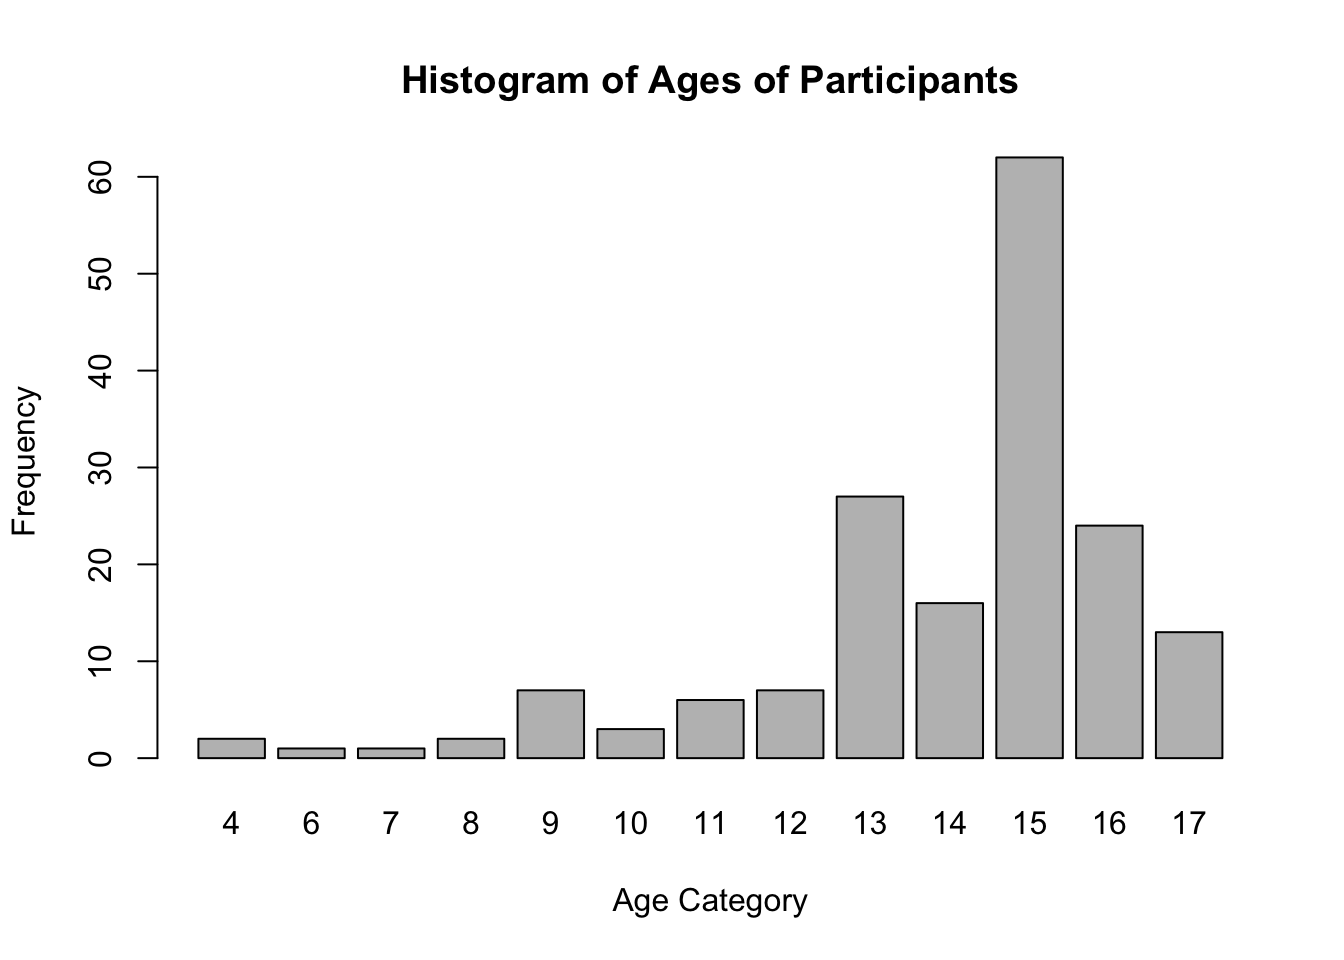
\includegraphics{Assignments_files/figure-latex/unnamed-chunk-20-1.pdf}

\emph{Answer: The age distribution of this sample is skewed left.
However, because the numbers within the data set are not actual ages,
but rather a range of ages or individual ages that are coded as numbers
1 through 17, we cannot base our true age distribution off of the
numbers that form the labels of the histogram. While it appears that the
Final Edited Age is skewed left, this may just be because the upper
coded ages contain wider ranges of ages, and the lower coded ages
contain only one or two ages.}

Do you think this age distribution representative of the US population?
Why or why not?

\emph{Answer: No, I do not believe this age distribution is
representative of the US population. According to Census data, and other
population pyramids that display the distribution of population, there
are many more younger people than are represented in this graph, as well
as many individuals outside of the scope of the study, such as those
under 12, etc. Even though (as I mentioned before) there are multiple
ages within certain categories, this data shows many more older
individuals compared to teenagers and those in their early twenties, and
Census data shows large numbers of those populations.}

Is the sample balanced in terms of gender? If not, are there more
females or males?

\begin{Shaded}
\begin{Highlighting}[]
\FunctionTok{table}\NormalTok{(dat}\SpecialCharTok{$}\NormalTok{irsex)}
\end{Highlighting}
\end{Shaded}

\begin{verbatim}
## 
##  1  2 
## 91 80
\end{verbatim}

1 (Male) 2 (Female) 91 80

\begin{Shaded}
\begin{Highlighting}[]
\NormalTok{counts }\OtherTok{\textless{}{-}} \FunctionTok{table}\NormalTok{(dat}\SpecialCharTok{$}\NormalTok{irsex)}
\FunctionTok{barplot}\NormalTok{(counts, }\AttributeTok{main =} \StringTok{"Gender Distribution"}\NormalTok{, }\AttributeTok{xlab =} \StringTok{"Gender"}\NormalTok{,}
    \AttributeTok{ylab =} \StringTok{"Frequency"}\NormalTok{, }\AttributeTok{names =} \FunctionTok{c}\NormalTok{(}\StringTok{"Male"}\NormalTok{, }\StringTok{"Female"}\NormalTok{))}
\end{Highlighting}
\end{Shaded}

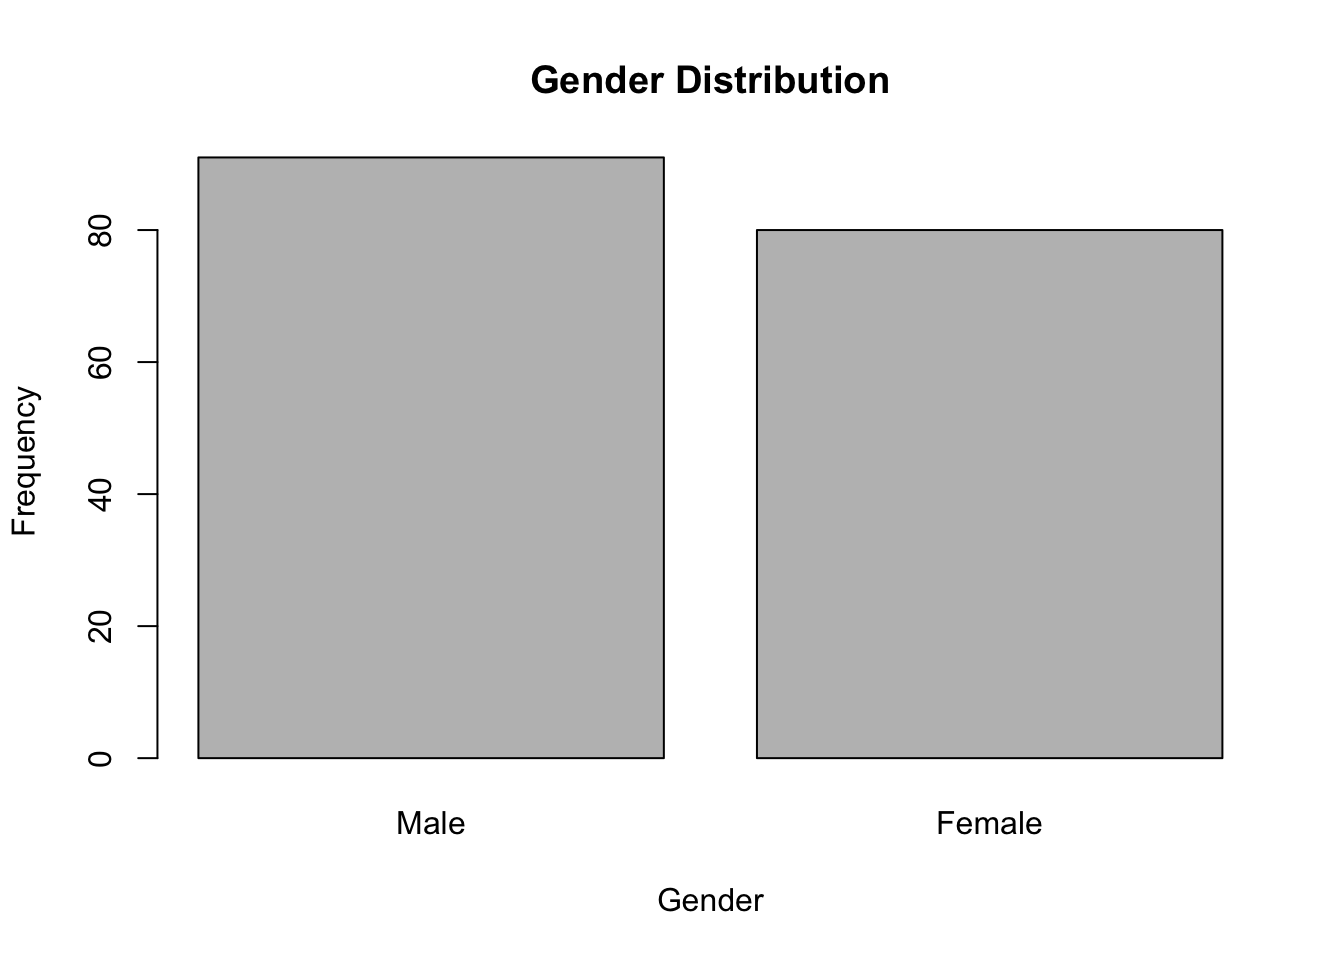
\includegraphics{Assignments_files/figure-latex/unnamed-chunk-22-1.pdf}

\emph{Answer: The sample is not gender balanced, as there are more males
(91) than females (80). Using a bar chart clearly demonstrates this
disparity.}

Use this code to draw a stacked bar plot to view the relationship
between sex and age. What can you conclude from this plot?

\begin{Shaded}
\begin{Highlighting}[]
\NormalTok{tab.agesex }\OtherTok{\textless{}{-}} \FunctionTok{table}\NormalTok{(dat}\SpecialCharTok{$}\NormalTok{irsex, dat}\SpecialCharTok{$}\NormalTok{age2)}
\FunctionTok{barplot}\NormalTok{(tab.agesex, }\AttributeTok{main =} \StringTok{"Age and Gender Comparison"}\NormalTok{, }\AttributeTok{xlab =} \StringTok{"Age Category"}\NormalTok{,}
    \AttributeTok{ylab =} \StringTok{"Frequency"}\NormalTok{, }\AttributeTok{legend.text =} \FunctionTok{c}\NormalTok{(}\StringTok{"Male"}\NormalTok{, }\StringTok{"Female"}\NormalTok{), }\AttributeTok{xlim =} \FunctionTok{c}\NormalTok{(}\DecValTok{0}\NormalTok{,}
        \DecValTok{17}\NormalTok{), }\AttributeTok{beside =} \ConstantTok{FALSE}\NormalTok{)  }\CommentTok{\# Stacked bars (default)}
\end{Highlighting}
\end{Shaded}

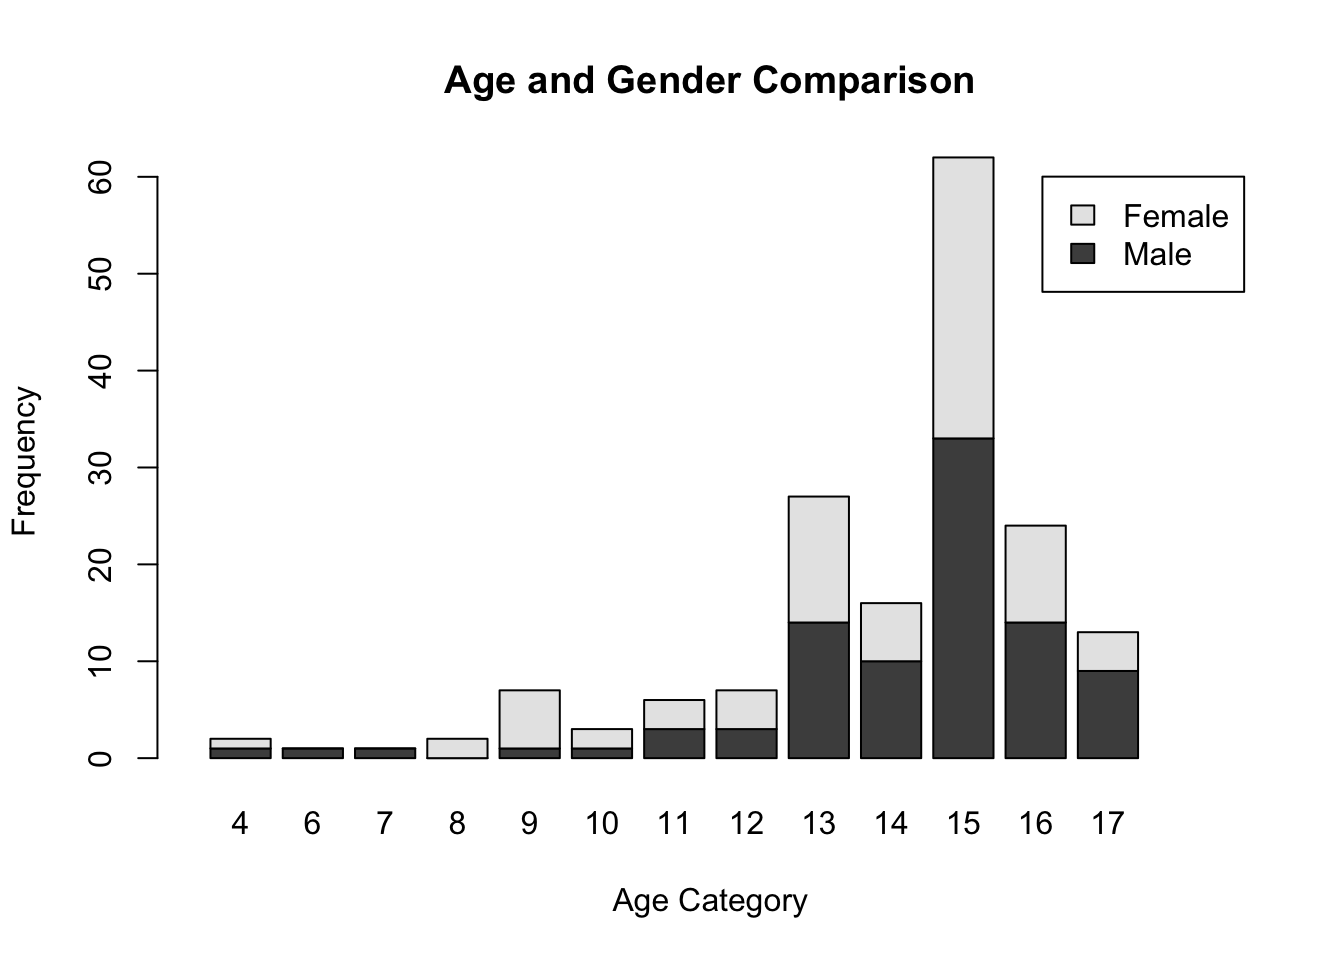
\includegraphics{Assignments_files/figure-latex/unnamed-chunk-23-1.pdf}

\emph{Answer: We can conclude from this plot that for most age
categories, there were more males than females. However, for age
categories 8, 9, 13, and 15, there appear to be more females or the same
number of males and females.}

\hypertarget{problem-4-substance-use}{%
\subsection{Problem 4: Substance use}\label{problem-4-substance-use}}

For which of the three substances included in the data set (marijuana,
alcohol, and cigarettes) do individuals tend to use the substance
earlier?

\begin{Shaded}
\begin{Highlighting}[]
\FunctionTok{par}\NormalTok{(}\AttributeTok{mfrow =} \FunctionTok{c}\NormalTok{(}\DecValTok{3}\NormalTok{, }\DecValTok{1}\NormalTok{))}
\FunctionTok{hist}\NormalTok{(dat}\SpecialCharTok{$}\NormalTok{mjage, }\AttributeTok{main =} \StringTok{"Histogram of Age of First Marijuana Use"}\NormalTok{,}
    \AttributeTok{xlab =} \StringTok{"Age Categories"}\NormalTok{, }\AttributeTok{ylab =} \StringTok{"Frequency"}\NormalTok{, }\AttributeTok{xlim =} \FunctionTok{c}\NormalTok{(}\DecValTok{0}\NormalTok{,}
        \DecValTok{50}\NormalTok{), }\AttributeTok{ylim =} \FunctionTok{c}\NormalTok{(}\DecValTok{0}\NormalTok{, }\DecValTok{50}\NormalTok{), }\AttributeTok{breaks =} \DecValTok{20}\NormalTok{)}
\FunctionTok{hist}\NormalTok{(dat}\SpecialCharTok{$}\NormalTok{iralcage, }\AttributeTok{main =} \StringTok{"Histogram of Age of First Alcohol Use"}\NormalTok{,}
    \AttributeTok{xlab =} \StringTok{"Age Categories"}\NormalTok{, }\AttributeTok{ylab =} \StringTok{"Frequency"}\NormalTok{, }\AttributeTok{xlim =} \FunctionTok{c}\NormalTok{(}\DecValTok{0}\NormalTok{,}
        \DecValTok{50}\NormalTok{), }\AttributeTok{ylim =} \FunctionTok{c}\NormalTok{(}\DecValTok{0}\NormalTok{, }\DecValTok{50}\NormalTok{), }\AttributeTok{breaks =} \DecValTok{20}\NormalTok{)}
\FunctionTok{hist}\NormalTok{(dat}\SpecialCharTok{$}\NormalTok{cigage, }\AttributeTok{main =} \StringTok{"Histogram of Age of Starting to Smoke Cigarettes Daily"}\NormalTok{,}
    \AttributeTok{xlab =} \StringTok{"Age Categories"}\NormalTok{, }\AttributeTok{ylab =} \StringTok{"Frequency"}\NormalTok{, }\AttributeTok{xlim =} \FunctionTok{c}\NormalTok{(}\DecValTok{0}\NormalTok{,}
        \DecValTok{50}\NormalTok{), }\AttributeTok{ylim =} \FunctionTok{c}\NormalTok{(}\DecValTok{0}\NormalTok{, }\DecValTok{50}\NormalTok{), }\AttributeTok{breaks =} \DecValTok{20}\NormalTok{)}
\end{Highlighting}
\end{Shaded}

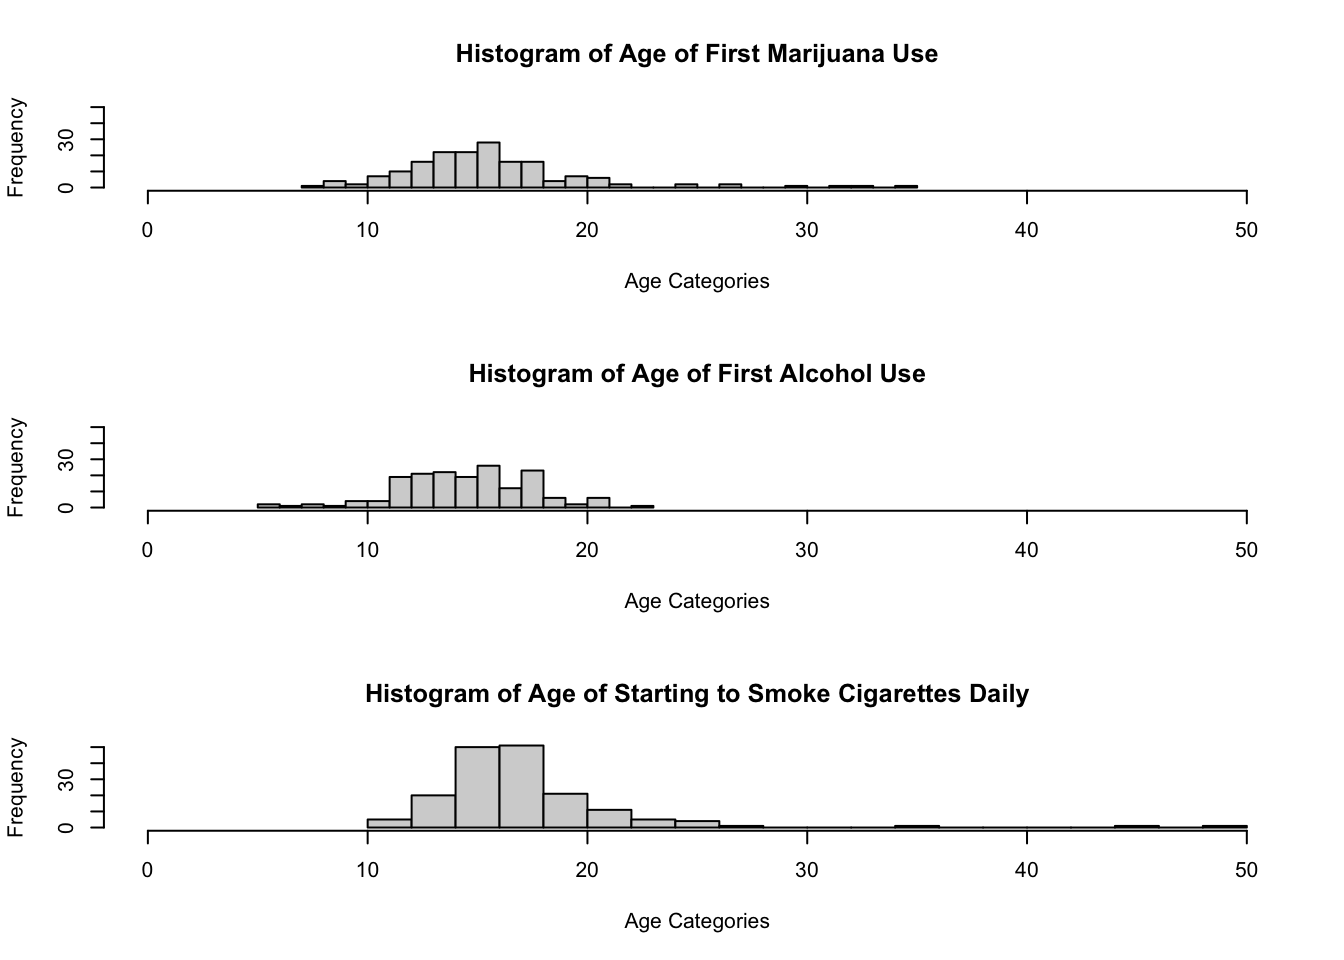
\includegraphics{Assignments_files/figure-latex/unnamed-chunk-24-1.pdf}

\emph{Individuals tend to use alcohol earlier, as seen on the
histograms.}

\hypertarget{problem-5-sexual-attraction}{%
\subsection{Problem 5: Sexual
attraction}\label{problem-5-sexual-attraction}}

What does the distribution of sexual attraction look like? Is this what
you expected?

\begin{Shaded}
\begin{Highlighting}[]
\NormalTok{dat1 }\OtherTok{\textless{}{-}}\NormalTok{ dat[dat}\SpecialCharTok{$}\NormalTok{sexatract }\SpecialCharTok{!=} \DecValTok{99}\NormalTok{, ]}
\NormalTok{counts1 }\OtherTok{\textless{}{-}} \FunctionTok{table}\NormalTok{(dat1}\SpecialCharTok{$}\NormalTok{sexatract)}
\FunctionTok{barplot}\NormalTok{(counts1, }\AttributeTok{main =} \StringTok{"Sexual Attraction Distribution"}\NormalTok{, }\AttributeTok{xlab =} \StringTok{"Sexual Attraction Categories"}\NormalTok{,}
    \AttributeTok{ylab =} \StringTok{"Frequency"}\NormalTok{, }\AttributeTok{ylim =} \FunctionTok{c}\NormalTok{(}\DecValTok{0}\NormalTok{, }\DecValTok{150}\NormalTok{))}
\end{Highlighting}
\end{Shaded}

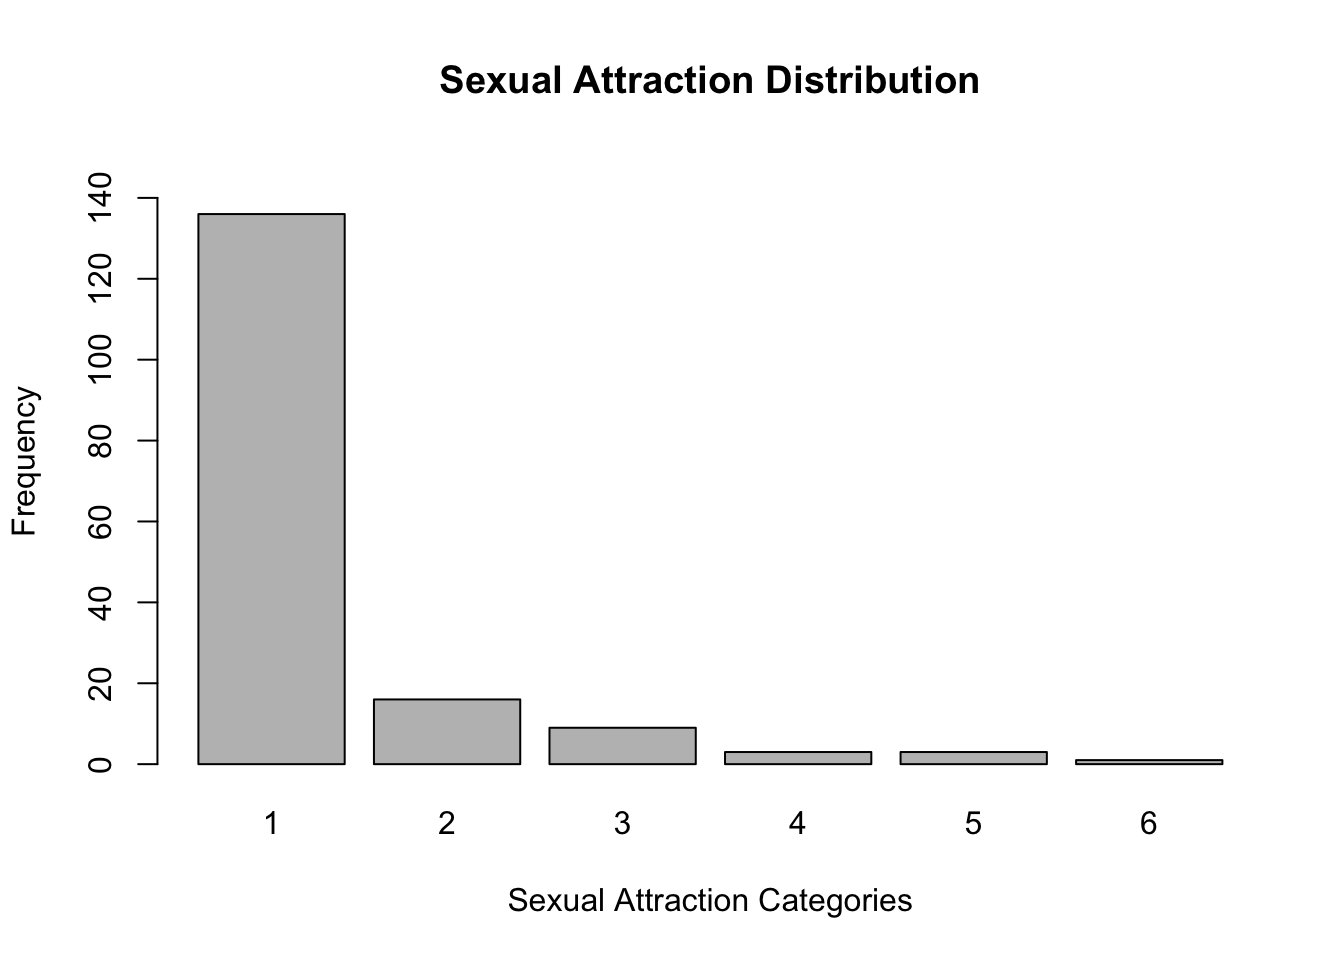
\includegraphics{Assignments_files/figure-latex/unnamed-chunk-25-1.pdf}

\emph{Answer: The distribution of sexual attraction is skewed right,
which is what I expected, as most people identify as only being
attracted to the opposite sex, with fewer people identifying as being
attracted to the same sex in any way. This is what I expected because I
believe that LGBT+ populations are still a relatively small minority
within the US compared to those who are only attracted to the opposite
sex.}

What is the distribution of sexual attraction by gender?

\begin{Shaded}
\begin{Highlighting}[]
\NormalTok{dat1 }\OtherTok{\textless{}{-}}\NormalTok{ dat[dat}\SpecialCharTok{$}\NormalTok{sexatract }\SpecialCharTok{!=} \DecValTok{99}\NormalTok{, ]}
\NormalTok{tab.sexor }\OtherTok{\textless{}{-}} \FunctionTok{table}\NormalTok{(dat1}\SpecialCharTok{$}\NormalTok{irsex, dat1}\SpecialCharTok{$}\NormalTok{sexatract)}
\FunctionTok{barplot}\NormalTok{(tab.sexor, }\AttributeTok{main =} \StringTok{"Sexual Attraction and Gender Comparison"}\NormalTok{,}
    \AttributeTok{xlab =} \StringTok{"Sexual Attraction Category"}\NormalTok{, }\AttributeTok{ylab =} \StringTok{"Frequency"}\NormalTok{,}
    \AttributeTok{legend.text =} \FunctionTok{c}\NormalTok{(}\StringTok{"Male"}\NormalTok{, }\StringTok{"Female"}\NormalTok{), }\AttributeTok{xlim =} \FunctionTok{c}\NormalTok{(}\DecValTok{0}\NormalTok{, }\DecValTok{7}\NormalTok{), }\AttributeTok{ylim =} \FunctionTok{c}\NormalTok{(}\DecValTok{0}\NormalTok{,}
        \DecValTok{140}\NormalTok{), }\AttributeTok{beside =} \ConstantTok{FALSE}\NormalTok{)  }\CommentTok{\# Stacked bars (default)}
\end{Highlighting}
\end{Shaded}

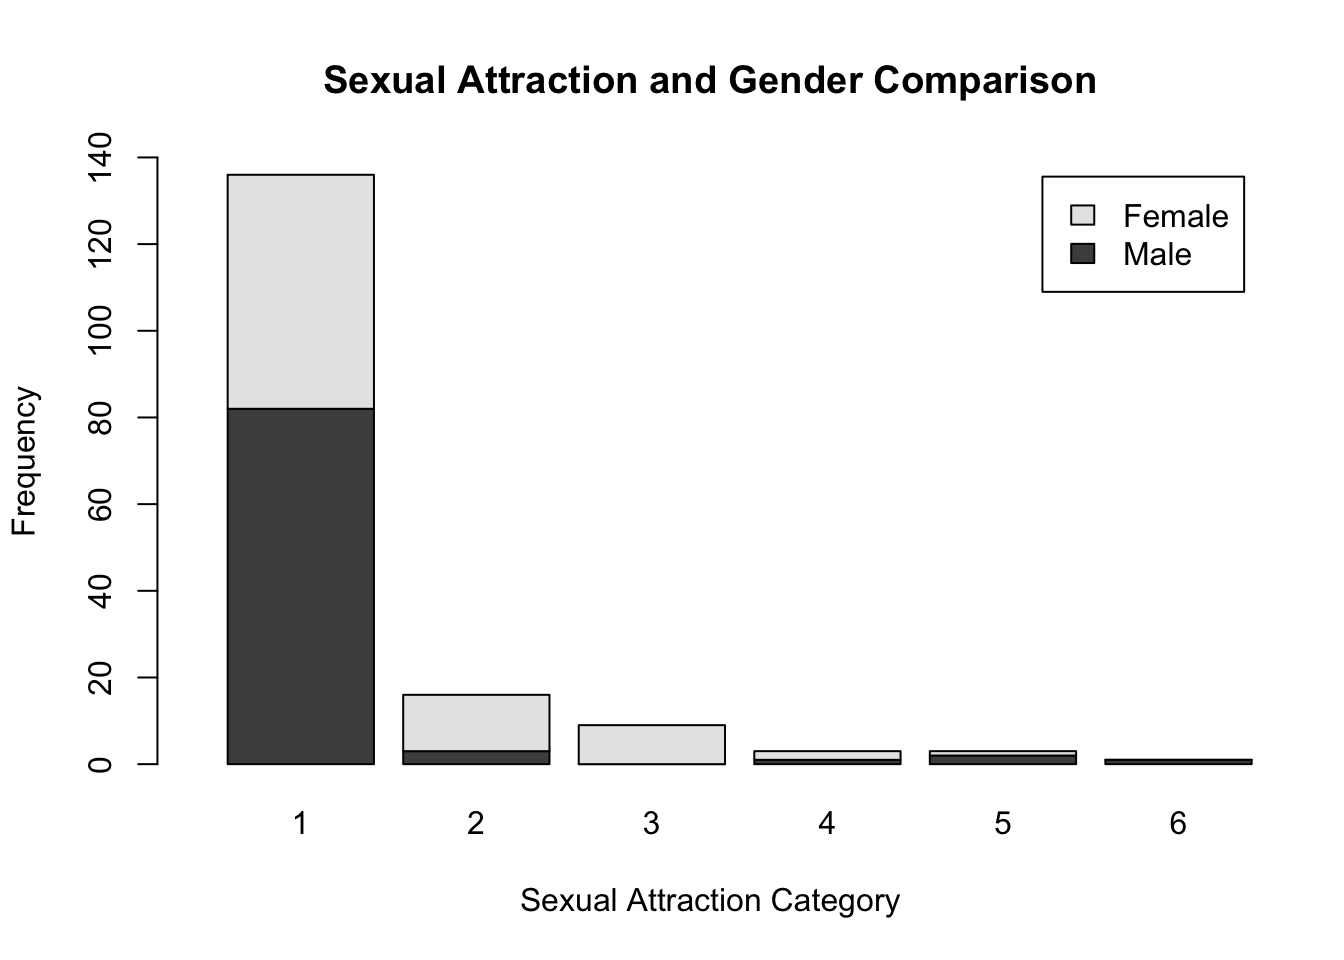
\includegraphics{Assignments_files/figure-latex/unnamed-chunk-26-1.pdf}

\emph{The distribution by gender is also skewed right, but there are
more females that identify with statements about being attracted to the
same sex in some way, and more males that identify with statements about
being attracted to the opposite sex, as can be seen in the stacked bar
chart.}

\hypertarget{problem-6-english-speaking}{%
\subsection{Problem 6: English
speaking}\label{problem-6-english-speaking}}

What does the distribution of English speaking look like in the sample?
Is this what you might expect for a random sample of the US population?

\begin{Shaded}
\begin{Highlighting}[]
\NormalTok{counts2 }\OtherTok{\textless{}{-}} \FunctionTok{table}\NormalTok{(dat}\SpecialCharTok{$}\NormalTok{speakengl)}
\FunctionTok{barplot}\NormalTok{(counts2, }\AttributeTok{main =} \StringTok{"English Language Category Frequency"}\NormalTok{,}
    \AttributeTok{xlab =} \StringTok{"English Speaking Categories"}\NormalTok{, }\AttributeTok{ylab =} \StringTok{"Frequency"}\NormalTok{,}
    \AttributeTok{ylim =} \FunctionTok{c}\NormalTok{(}\DecValTok{0}\NormalTok{, }\DecValTok{200}\NormalTok{))}
\end{Highlighting}
\end{Shaded}

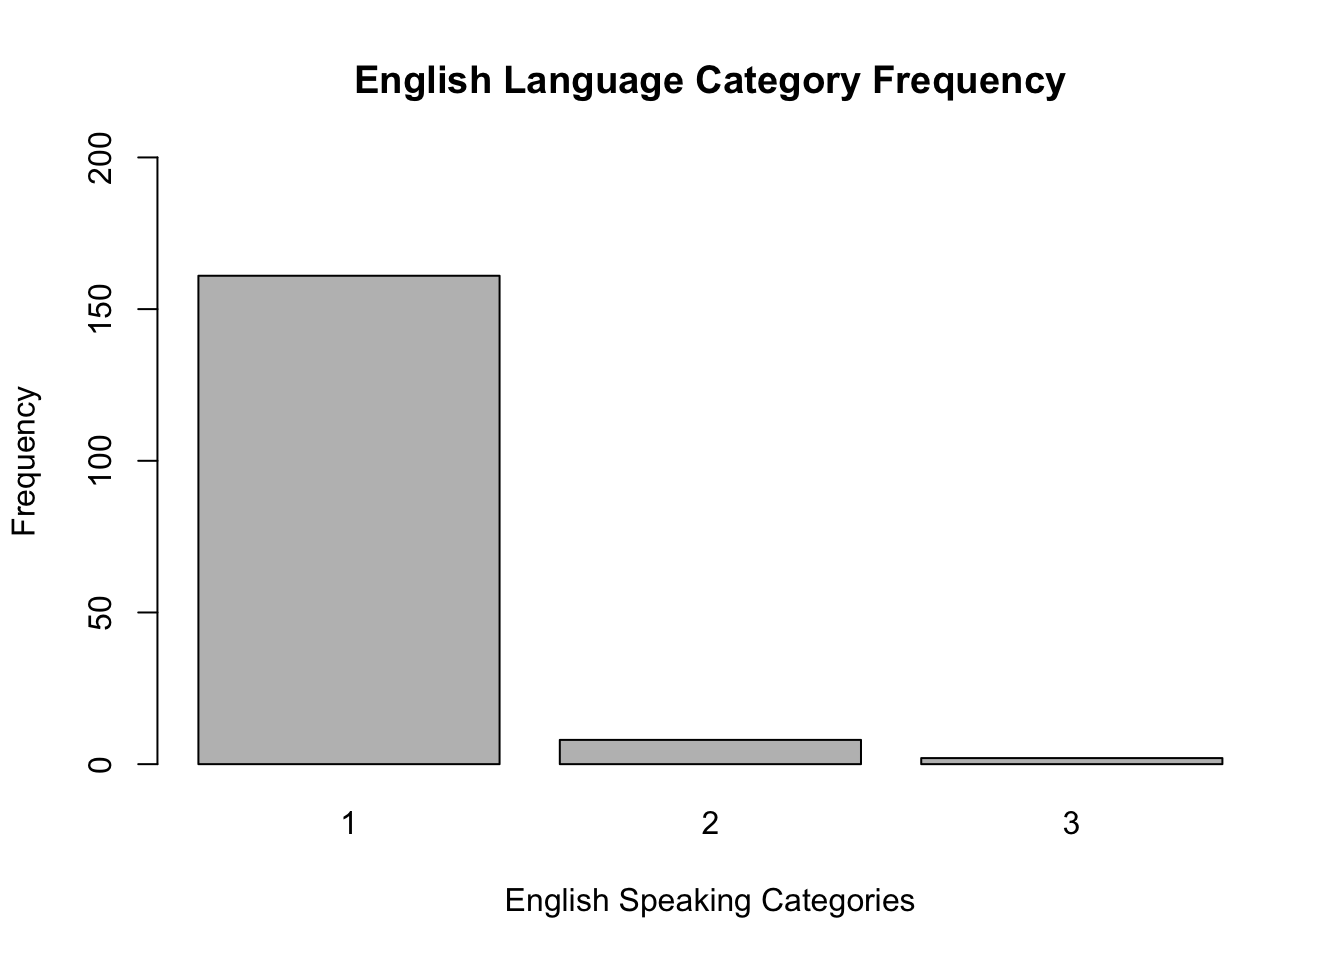
\includegraphics{Assignments_files/figure-latex/unnamed-chunk-27-1.pdf}

\emph{This distribution is also skewed right, with most individuals
responding that they speak English very well, and less than 50
individuals total saying that the speak English well or not well, and
nobody saying they did not speak English at all. This is similar to the
distribution that I would expect in the United States because even
though the US has no official language, most people need to speak some
English in order to work and live here. However, there are probably more
people in the US that speak no English at all, but they just were not
able to participate in the survey because it was conducted in English.}

Are there more English speaker females or males?

\begin{Shaded}
\begin{Highlighting}[]
\FunctionTok{table}\NormalTok{(dat}\SpecialCharTok{$}\NormalTok{irsex, dat}\SpecialCharTok{$}\NormalTok{speakengl)}
\end{Highlighting}
\end{Shaded}

\begin{verbatim}
##    
##      1  2  3
##   1 84  7  0
##   2 77  1  2
\end{verbatim}

\begin{Shaded}
\begin{Highlighting}[]
\NormalTok{tab.sexor }\OtherTok{\textless{}{-}} \FunctionTok{table}\NormalTok{(dat}\SpecialCharTok{$}\NormalTok{irsex, dat}\SpecialCharTok{$}\NormalTok{speakengl)}
\FunctionTok{barplot}\NormalTok{(tab.sexor, }\AttributeTok{main =} \StringTok{"English Skill and Gender Comparison"}\NormalTok{,}
    \AttributeTok{xlab =} \StringTok{"English Ability Category"}\NormalTok{, }\AttributeTok{ylab =} \StringTok{"Frequency"}\NormalTok{, }\AttributeTok{legend.text =} \FunctionTok{c}\NormalTok{(}\StringTok{"Male"}\NormalTok{,}
        \StringTok{"Female"}\NormalTok{), }\AttributeTok{xlim =} \FunctionTok{c}\NormalTok{(}\DecValTok{0}\NormalTok{, }\DecValTok{4}\NormalTok{), }\AttributeTok{ylim =} \FunctionTok{c}\NormalTok{(}\DecValTok{0}\NormalTok{, }\DecValTok{200}\NormalTok{), }\AttributeTok{beside =} \ConstantTok{FALSE}\NormalTok{)  }\CommentTok{\# Stacked bars (default)}
\end{Highlighting}
\end{Shaded}

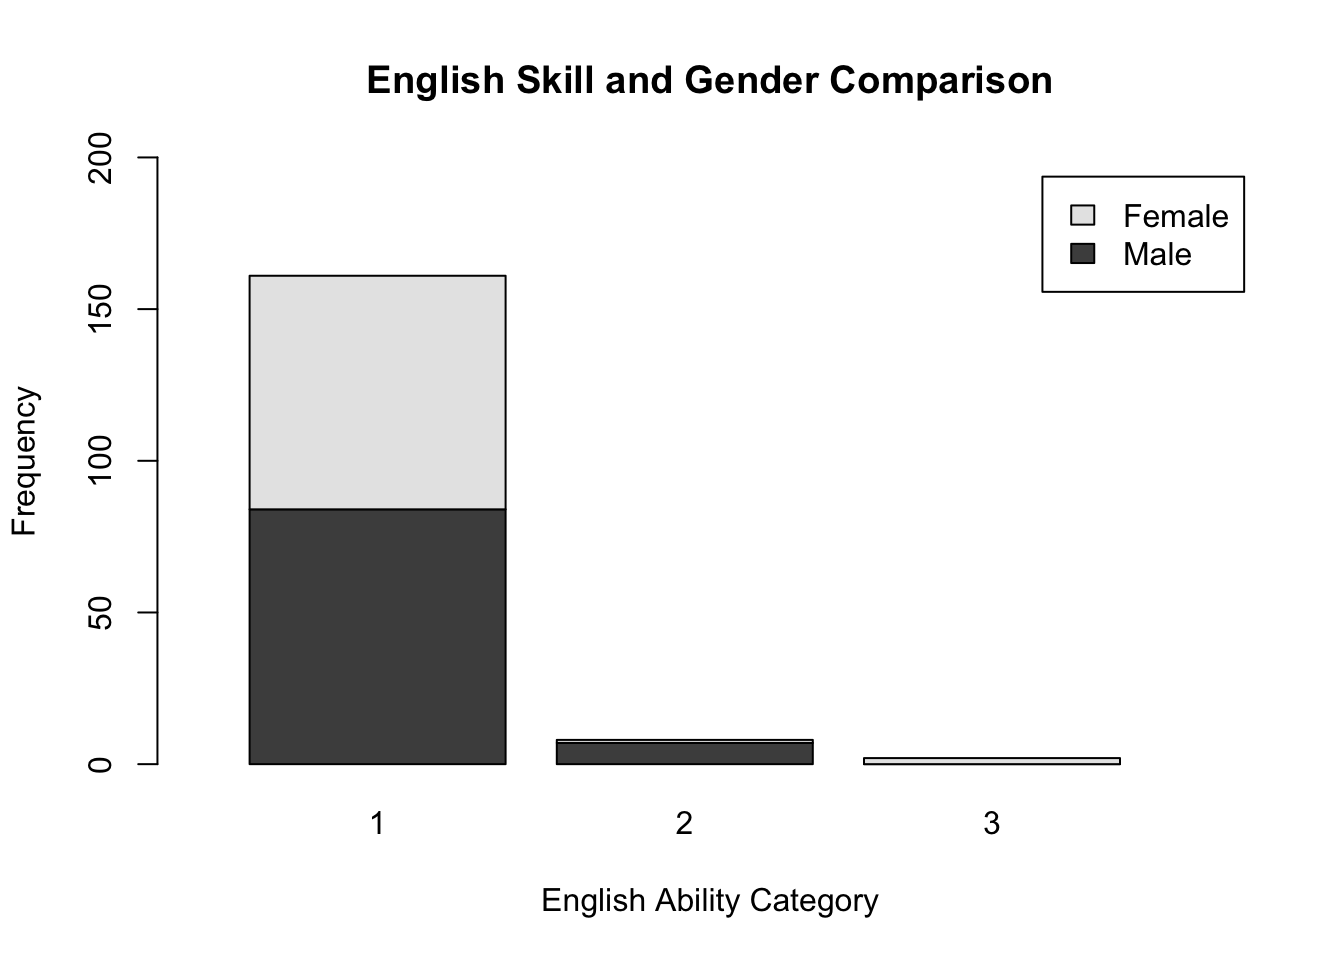
\includegraphics{Assignments_files/figure-latex/unnamed-chunk-28-1.pdf}

\emph{There are more male English speakers than female English speakers,
but that might also be due to the fact that there are more males than
females within the data set to begin with.}

\[\\[2in]\]

\end{document}
